\section{Halvledare} 

\footnote{Videor relevanta till kapitel \ref{sec:halvledare}: \href{https://www.youtube.com/playlist?list=PL2ub1_oKCn7ogaMtdB2RumlIYqNeXf_oX}{Khan Academy, Semiconductors, videor 5-9.}}
\label{sec:halvledare}
Halvledare kallas det för att de kan både leda, och isolera\footnote{Fräckt!}. Vid låg temperatur kommer halvledaren att isolera och vid hög temperatur kommer den att leda bättre. Vad som är hög och låg temperatur är unikt för varje enskilt ämne. När man ökar temperaturen kring en halvledare och dess ledningsförmåga ökar, kommer elektronerna i ämnet att börja hoppa från det helt fyllda valensbandet över till ledningsbandet. En elektron som hoppar till ledningsbandet (eller tvärtom) lämnar ett hål bakom sig på platsen den lämnade. Dessa hål är inte partiklar men det är intuitivt att se dem som partiklar som rör sig i motsatt riktning från elektronernas rörelse. Föreställ dig en nästan fylld vattenflaska med en luftbubbla i sig. Håller du flaskan upprätt kommer allt vatten sjunka till botten (och luftbubblan lägger sig överst i flaskan). Vänder du flaskan upp och ner kommer allt vatten att lägga sig vid flaskans lock, och luftbubblan lägga sig vid flaskans botten (numera ovansidan). Luftbubblans rörelse provoceras som en följd av vattnets rörelse. 
\begin{figure}[ht]
    \centering
    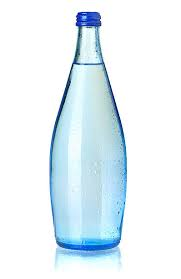
\includegraphics[scale = 0.3]{bilder/vatten.png}
    \caption{Flaska, möjligtvis av glas, fylld med genomskinlig vätska.}
    \label{fig:vatten}
\end{figure}

\subsection{Extrinsiska halvledare, doping}

\textbf{Definition:} En halvledare kallas 'intrinsisk' om alla atomer är av samma ämne \footnote{Intrinsiska halvledare kallas ibland 'pura' halvledare.}. Motsatsen gäller även, alltså; en halvledare bestående av mer än ett ämne kallas 'extrinsiska'.

Då du kombinerar två ämnen kommer det att påverka dess elektronstruktur. Mellan den intrinsiska halvledarens valensband och ledningsband kommer en ny möjlig energinivå att dyka upp. Elektroner kan hoppa till denna nya energinivå. Är den nya nivån nära valensbandet kommer den att uppmuntra elektronerna i valensbandet att hoppa dit, och således lämna hål efter sig i valensbandet. Vice versa gäller för om den nya energinivån ligger nära ledningsbandet.

För en p-typ halvledare kallas den nyuppståndna energinivån acceptornivå. Om du dopar din halvledare med ett ämne som ligger i atomgruppen nedanför kommer acceptornivån ligga precis ovanför valensbandet, vilket gör det sannolikt för elektroner att hoppa dit. Ju längre ner i atomgrupperna du går, desto längre bort från valensbandet hamnar denna acceptornivå, och minskar alltså den önskade effekten av att skapa hål i valensbandet.

Motsvarande gäller även för n-typ halvledare, fast ju längre uppåt i atomgrupperna du vandrar, desto närmare valensbandet kommer du med acceptornivån, vilket minskar valensbandets elektronkoncentration, alltså motsatt från önskad effekt.

T.ex kisel tillhör atomgrupp 14. Kombinerar du kisel med ett ämne från atomgrupp 15, alltså med en elektron mer än kisel, kommer den atomen, efter sina kovalenta bindningar, ha en elektron över som inte är bunden. Den elektronen är fri. Detta kommer leda till ett 'överflöd' av elektroner i valensbandet, och ämnets ledningsförmåga ökar avsevärt. Ämnet med många elektroner kallas för en 'n-typ halvledare'.

Omvänt gäller; om du dopar ett ämne (gör ämnet extrinsiskt) med ett ämne från atomgruppen under, så kommer det att skapas en stor mängd hål i valensbandet, vilket 

\subsection{PN-övergång}

Då två p-dopade resp. n-dopade halvledare sätts ihop bildas en PN-övergång. Området i mitten av de två halvledarna kallas för spärrskikt, där de respektive majoritetsladdningsbärarna tar ut varandra i vad som kallas rekombination. Med hjälp av en PN-övergång och manipulation av dess spärrskikt kan man få PN-övergången att fungera som en diod.

\subsection{Dioder}
Denna ovannämnda manipulation består av att 'framspänna' PN-övergången. Detta innebär att man tillför en spänningskälla, en förspänning, vars positiva sida är kopplad till PN-föreningens (diodens) positiva sida, och motsvarande för de negativa sidorna. Då källans spänning ökar kommer spärrskiktet kontinuerligt att minska tills det inte finns längre, och dioden fungerar då som en väldigt bra ledare. Spänningen då spärrskiktet är minskat till noll kallas för diodens tröskelspänning. Man kan även invertera källans poler och då 'backspänna' dioden. Man kan även säga att man 'biaserar' dioden (positivt eller negativt).

Om du byter backspänner dioden kommer du uppnå motsatt effekt, alltså att spärrskiktet bara ökar i storlek. Slutsatsen blir att dioden bara släpper igenom ström då spänningen har 'rätt' polaritet, vilket ger oss en mycket användbar komponent i kretsdesign, till exempel vid implementering av \href{https://sv.wikipedia.org/wiki/Likriktning}{likriktare}.

\begin{figure}[ht]
    \centering
    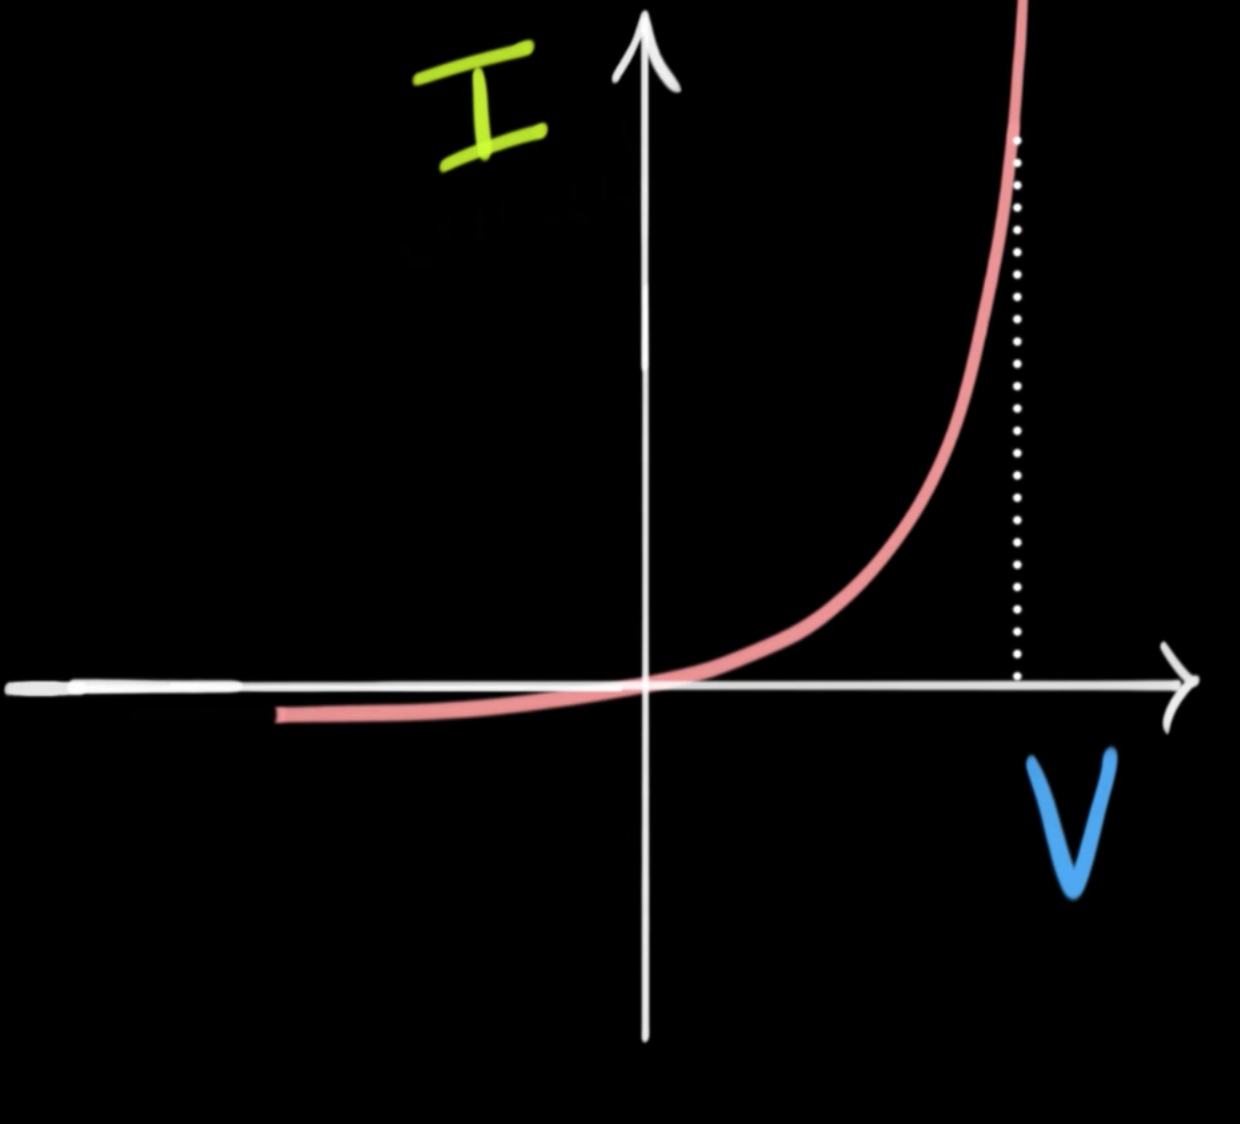
\includegraphics[scale = 0.3]{bilder/fig: arbetspunkt.png}
    \caption{Ström som flödar genom en diod plottat mot dess förspänning. Vita punkterna visar diodens arbetspunkt, dess tröskelspänning.}
    \label{fig:arbetspunkt}
\end{figure}

\newpage

Resten av kursen består av elektronik kopplat till transistorer. Jag har inte mer tid och förhoppningsvis har du lärt dig hur en transistor fungerar någorlunda i tidigare elektronikkurser, därför kommer jag för denna gång att avsluta sammanfattningen av denna fina kurs här! 

